\documentclass[a4paper,12pt]{article}
\usepackage[utf8]{inputenc}
\usepackage[brazil]{babel}
\usepackage{amsmath,amsfonts,amssymb,amsthm,dsfont,mathtools}
\usepackage{blindtext}
\usepackage{graphicx}

\title{Trabalho de Álgebra Linear - Análise de dados utilizando PCA}
\author{Luiz Felipe Pierre Pestana \\ Gabriel Andrade Nascimento}

\date{Dezembro de 2022}

\begin{document}

\maketitle

\section{DataSet}
    \par Foi selecionado um dataset da Hass Avocado Board sobre o preço médio de abacates em regiões dos EUA. A dataset representa os dados de varredura de varejo semanais de 2018 para volume de varejo nacional (unidades) e preço. Os dados de varredura do varejo vêm diretamente das caixas registradoras dos varejistas com base nas vendas reais no varejo de abacates Hass.
    Este dataset possui diversas variáveis, como: Preço Médio, Volume Total, Data,etc.
\section{Algoritmo}
    Primeiro, foram descartadas as colunas que eram do tipo string, pois não teriam utilidade para o algoritmo.
\begin{verbatim}
df_drop = df.drop(labels=['Unnamed: 0','Date','type','region'], axis=1)
\end{verbatim}
    Após isso, os dados foram normalizados, encontrando a média(mean) e subtraindo pelo
    total de dados.Com isso, os dados das colunas ficam mais uniformes.
\begin{verbatim}
    mean = np.mean(df_drop,axis=0)
    mRd = df_drop - mean
\end{verbatim}
    Então foi calculada a matriz de covariância, sendo transposta para que o algoritmo trabalhasse com as colunas ao invés da linhas.
\begin{verbatim}
    cov_matrix = np.cov(mRd.T)
\end{verbatim}
    Com a matriz de covariância já calculada, deve-se encontrar os autovalores e autovetores. Após calculados, eles foram colocados em ordem, afim de se descobrir quais são os dois maiores autovalores.
\begin{verbatim}
    autval,autvet = np.linalg.eig(cov_matrix)
    autval = np.array(np.sort(autval[::-1]))
\end{verbatim}
    Os dois maiores autovalores encontrados foram de 1.41871133e+11 e 1.63121576e+13 que correspondem ás colunas Average Price(Preço Médio em Dólar) e Total Volume(Volume total de venda).
    Então foi feito um gráfico para representar essas colunas.
\begin{verbatim}
    sns.lineplot(x=df_drop.columns[0],y=df_drop.columns[1],
    data=df_drop)
    plt.show()
\end{verbatim}
\begin{figure}[h]
    \caption{Gráfico do maiores autovalores}
    \centering
    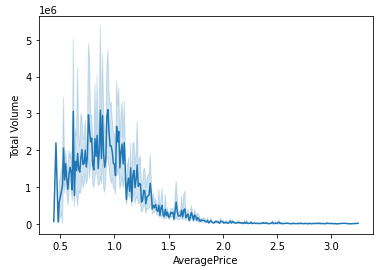
\includegraphics{figura/image.png}
    \label{figura:my_label}
\end{figure}
    Ao observar o gráfico, nota-se uma maior concentração do volume total de vendas, onde o preço médio do abacate variou entre 0.5 e 1 dólar.


\end{document}
